\documentclass[10pt]{article}
\usepackage[usenames]{color} %used for font color
\usepackage{amssymb} %maths
\usepackage{amsmath} %maths
\usepackage[utf8]{inputenc} %useful to type directly diacritic characters
\usepackage[letterpaper, portrait, margin=1.5in]{geometry}
\usepackage{graphicx,wrapfig}
\usepackage{booktabs}
\usepackage{multicol}
\begin{document}
\subsection*{MSDS650 Week 5 Assignment - Nathan Worsham}
RapidMiner is something completely new to me. I started this week with watching several videos. I generally prefer to work with code as opposed to a GUI, so RapidMiner is a bit of a challenge for me. It seems that the product has many coding concepts in it (i.e. branch, loop, output, input, etc) but one must drag and drop and connect graphical representations to get it to run the process. It can be very confusing as for which to connect to what as the inputs and outputs are often abbreviations. I found it to be very buggy as several times I received exceptions. Starting off following the example I wasn't even sure where to find "Process Documents from Files", but after poking around for awhile realized that  the Operators section has a search feature and found that the option existed in the package I was instructed to download earlier. Once I was finished with the simple example I began to explore. Having the word list to compare the two documents (tweets and job listings), clicking on the "Document Occurrences" column I could see that from the word list produced, that only 12 words were in common between the 2 documents.
\begin{figure}[!h]
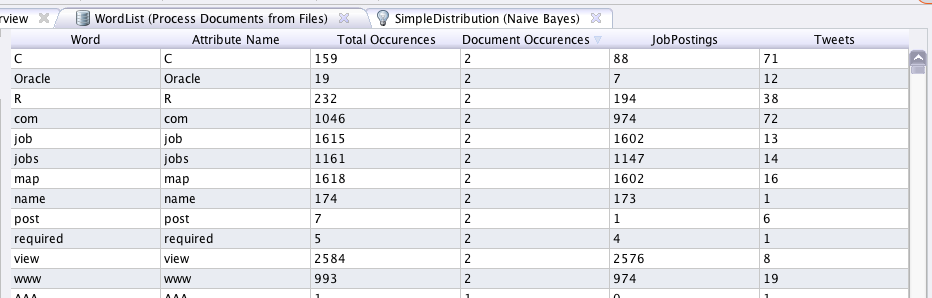
\includegraphics[scale=0.37]{wordlist_incommon.png}
\centering
\end{figure}\\
Next I added the "Transformation Cases" operator to change all words to lowercase, this changed to the common words between documents to 15. Now I was more interested in exploring the documents individually rather than comparing them with each other by first seeing the top words for each document. By simply clicking on the column headers, I could see the top words for each document. For the tweets there were a lot of single and double character results, so I added "Filter Tokens (by Length)" operator to get its count, removing 1 and 2 character words.
\begin{multicols}{2}
Job Postings
\begin{verbatim}
view	2576
trk	1775
browse	1602
job	1602
map	1602
jobs	1147
linkedin	975
com	974
https	974
www	974
\end{verbatim}
Tweets
\begin{verbatim}
false	2813
finalized	2811
http	2448
information	2327
co	2137
nestle	1228
pfizer	897
action	864
citi	663
news	609
\end{verbatim}
\end{multicols}
From the assignment, I did the "Naive Bayes" operator. The chart that it provided basically always looks like normal curves and lets you compare words graphed against each other. Using an example of a word that exists in both documents--oracle--the graphs completely overlap. Using an example of a top word in one document and non-existent in the other--false--the graphs look much further apart then the majority of the other words I clicked on. 
\par
\raisebox{-.5\height}{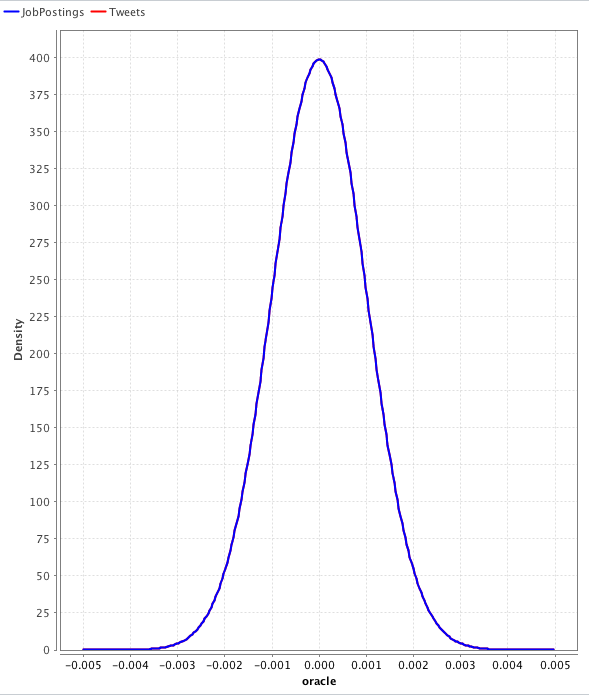
\includegraphics[width=7cm]{oracle.png}}%
\hfill
\raisebox{-.5\height}{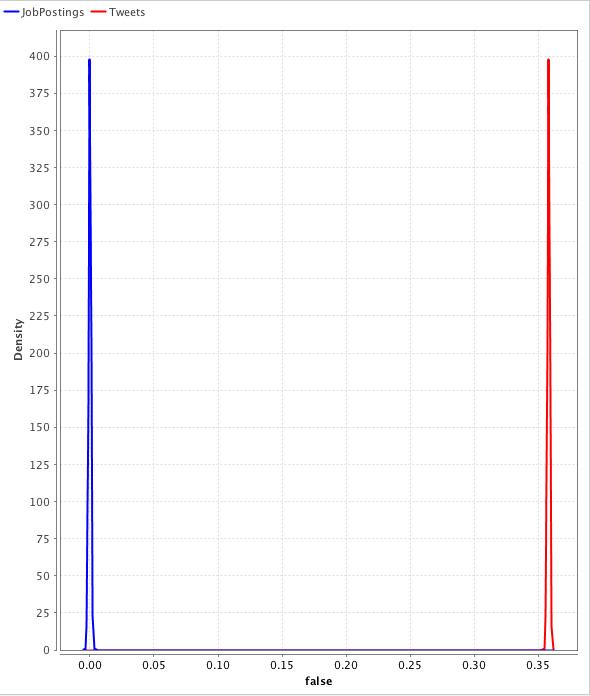
\includegraphics[width=7cm]{false.png}}%
\par
Next, following along with the video instruction provided from part I, I was interested in capturing n-grams. Trying to understand exactly what are n-grams, Wikipedia (n.d.) has a decent definition of "an n-gram is a contiguous sequence of n items from a given sequence of text or speech". But watching a Coursera video on "Introduction to N-grams" explains that they can be used to compute the probability of a sentence or sequence of words, which can help with summarization, speech recognition, spell checks, and auto translations. What I found is really interesting to play with is Google's ngram viewer which can show the popularity of ngrams from books graphed against each other (https://books.google.com/ngrams). Anyway to generate the n-grams I enabled the "Generate n-Grams (Terms)" operator and started by setting it to a max length of 3. I wasn't really sure how to get RapidMiner to filter the results to just 2 or 3 grams so instead I elected to export to a csv to accomplish this. I found I needed to add 2 operators--"Wordlist to Data" and "Write CSV"--to get it to work. Once I had the csv file I used grep to create a new document with only ngrams over 1 since RapidMiner connects them with underscores:
\begin{verbatim}
cat week5_results_ngram.csv |grep _ > week5_results_ngram_filtered.csv
\end{verbatim}
Then I could simply use a spreadsheet editor to sort the data by specific columns. Now viewing the top ten n-grams I start to see the previous top ten single words appearing together and the Job Postings data is really starting to just look like portions of a URL address. 
\pagebreak
\begin{multicols}{2}
Job Postings
\begin{verbatim}
browse_map	1602
job_view	1602
job_view_browse	1602
trk_job	1602
trk_job_view	1602
view_browse	1602
view_browse_map	1602
com_jobs	974
com_jobs_view	974
https_www	974
\end{verbatim}
Tweets
\begin{verbatim}
false_finalized	2811
http_co	2122
false_finalized_information	1938
finalized_information	1938
false_finalized_action	628
finalized_action	628
pfizer_news	586
information_nestle	577
finalized_information_nestle	479
information_pfizer	450
\end{verbatim}
\end{multicols}
Trying to follow right along with the example from the videos from the assignment, I was not able to get the association rules to work. I found that I could get it to work all the way up to "FP-Growth". But after trying to run the process with the "Create Association Rules" I would always receive a Java error:
\begin{figure}[!h]
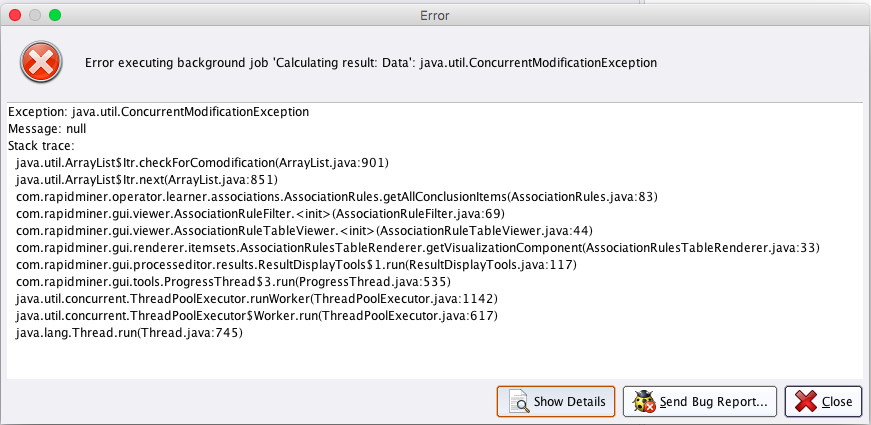
\includegraphics[scale=0.33]{java_exception.png}
\centering
\end{figure}
\\*
I tried changing the values from the operators leading up, like stopping FP-Growth from only finding a max of 5 to no avail and then I tried changing the confidence level on the association rules. I found that if I moved the confidence level down I would receive messages about it is trying to use too much memory which would require a full license. I decided to give it one last chance by changing the way my data came in--I loaded one of the csv's into a local repository and then used "Retrieve Data" and "Process Documents from Data" operators--but I still received the same error.
\begin{figure}[!h]
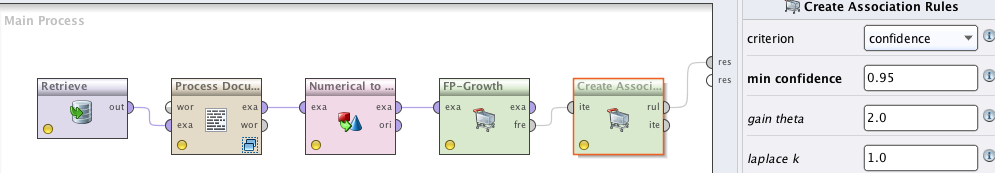
\includegraphics[scale=0.37]{altFail.png}
\centering
\end{figure}\\
I feel I wasted too much time trying to get this to work and really felt quite lost on what else I should try besides this afterward. So trying to move on, I decided to try out the "Stem (Porter)" operator to see if my results would look any different:
\begin{multicols}{2}
Job Postings
\begin{verbatim}
job	2749
view	2576
trk	1775
brows	1602
map	1602
linkedin	975
com	974
http	974
www	974
ye	974
\end{verbatim}
Tweets
\begin{verbatim}
final	2820
fals	2813
http	2448
inform	2330
co	2137
nestl	1229
pfizer	897
action	865
citi	706
new	609
\end{verbatim}
\end{multicols}
The results look only slightly different from the original top words from each document. 


\subsection*{References}
Wikipedia.com, n.d. Retrieved from https://en.wikipedia.org/wiki/N-gram\\
Coursera.com. Retrieved from https://class.coursera.org/nlp/lecture/14
\end{document}
